	
%% Informacje podstawowe
	\documentclass[10pt, twoside, fleqn]{article}
	\usepackage[a4paper, left=2.5cm, right=2.5cm, top=2.5cm, bottom=2.5cm, headsep=1.2cm]{geometry}

%% Ustawienia językowe
	\usepackage[UKenglish,polish]{babel}
	\usepackage{polski}
	\usepackage[utf8]{inputenc}

\def\mydate{\leavevmode\hbox{\twodigits\day.\twodigits\month.\the\year}}
\def\twodigits#1{\ifnum#1<10 0\fi\the#1}

\usepackage{array}
\newcolumntype{M}[1]{>{\centering\arraybackslash}m{#1}}
\newcolumntype{N}{@{}m{0pt}@{}}
\usepackage[table]{xcolor}
\usepackage{hhline}

%% Klikalny spis treści (usunąć do wersji do druku)
%\usepackage{hyperref}
%\hypersetup{
%    colorlinks=true,
%    linkcolor=blue,
%    filecolor=magenta,      
%    urlcolor=blue,
%}


%% Obrazki
	\usepackage{graphicx}
	\usepackage{wrapfig}
	\usepackage[export]{adjustbox}
	\usepackage{subcaption}

%% wykresy
	\usepackage{tikz}
	\usetikzlibrary{datavisualization}
	\usetikzlibrary{datavisualization.formats.functions}


%% Dodatki matematyczne
	\usepackage{amsmath}	
	\setlength{\mathindent}{0pt}
	\usepackage{esvect}			%wektory \vv - ladniejsze niz standardowe
	\usepackage{gensymb}		%\degree

%% obsluga kolumn w dokumencie
	\usepackage{multicol}


%% ładniejsze pierwiastki
	\usepackage{letltxmacro}
	\makeatletter
	\let\oldr@@t\r@@t
	\def\r@@t#1#2{%
	\setbox0=\hbox{$\oldr@@t#1{#2\,}$}\dimen0=\ht0
	\advance\dimen0-0.2\ht0
	\setbox2=\hbox{\vrule height\ht0 depth -\dimen0}%
	{\box0\lower0.4pt\box2}}
	\LetLtxMacro{\oldsqrt}{\sqrt}
	\renewcommand*{\sqrt}[2][\ ]{\oldsqrt[#1]{#2}}
	\makeatother

%% Metadata PDF zapisywanie
	\usepackage{ifpdf}
	\ifpdf
	\pdfinfo{
	   /Author (Piotr Choczynski)
	   /Title (Zestaw wzorów) }

%% Podstawowe informacje
	\title{Zestaw wzorów}
	\author{Piotr Choczyński}

%%	Nagłówek
	\usepackage{fancyhdr}
	\pagestyle{fancy}
		\fancyhead[RE,LO]{\rightmark}
		%\lhead{\rightmark}
	\chead{}
		\fancyhead[LE,RO]{\textbf{ZESTAW WZORÓW}}
		%\rhead{\textit{Piotr Choczyński} (p.j.choczynski@wp.pl)}
	\lfoot{}
	\cfoot{}
		\fancyfoot[RE,LO]{\thepage}
		\fancyfoot[RO]{\textit{Piotr Choczyński} (p.j.choczynski@wp.pl) \hspace{10pt} \LaTeX}
		\fancyfoot[LE]{\LaTeX \hspace{10pt} \textit{Piotr Choczyński} (p.j.choczynski@wp.pl)}
		%\rfoot{\LaTeX}
	\renewcommand{\headrulewidth}{0.4pt}
	\renewcommand{\footrulewidth}{0.4pt}
	\renewcommand{\sectionmark}[1]{\markright{#1}}
	\renewcommand{\subsectionmark}[1]{}


%%	Definicje funkcji matematycznych
	\DeclareMathOperator{\arctg}{arctg}
	\DeclareMathOperator{\arcctg}{arcctg}
	
	\setlength{\intextsep}{0mm}

%----------------------------------------------------------------------------------------
%	TITLE PAGE
%----------------------------------------------------------------------------------------

\newcommand*{\titleGM}{\begingroup % Create the command for including the title page in the document
\hbox{ % Horizontal box
\hspace*{0.2\textwidth} % Whitespace to the left of the title page
\rule{1pt}{\textheight} % Vertical line
\hspace*{0.05\textwidth} % Whitespace between the vertical line and title page text
\parbox[b]{0.75\textwidth}{ % Paragraph box which restricts text to less than the width of the page

{\noindent\Huge\bfseries Zestaw wybranych wzorów matematycznych} 

\vspace{25pt}
\hrule 
\vspace{25pt}

{\Large \textbf{\textit{matematyka elementarna}}}\\[1\baselineskip]
{\Large \textbf{\textit{pochodne}}}\\[1\baselineskip]
{\Large \textbf{\textit{całki}}}\\[1\baselineskip]
{\Large \textbf{\textit{geometria analityczna w 3D}}}\\[1\baselineskip]
{\Large \textbf{\textit{elementy trygonometrii sferycznej}}}

\vspace{25pt}
\hrule 
\vspace{25pt}

%----do klikalnych linków----%
%{\LARGE \textbf{Piotr Choczyński}}				\\[1\baselineskip]
%{\LARGE \text{\href{mailto:p.j.choczynski@wp.pl}
%			 {p.j.choczynski@wp.pl}}}			\\[1\baselineskip]
%{\large	\textit{\hyperlink{www.e-korepetycje.net/pjchocz}
%						  {www.e-korepetycje.net/pjchocz}}}
%----------------------------%


%----do wersji do druku------%
{\Large \textbf{Piotr Choczyński}}				\\[1\baselineskip]
{\Large \text{p.j.choczynski@wp.pl}}			\\[1\baselineskip]
{		\textit{www.e-korepetycje.net/pjchocz}}
%----------------------------%


\vspace{0.4\textheight}
%	\begin{flushright}
\raggedleft
		\Large\textit{\mydate \hspace{10pt} v2.2} 
%	end{flushright}
}}
\endgroup}

%----------------------------------------------------------------------------------------
%----------------------------------------------------------------------------------------


\begin{document}


	%Strona tytułowa
	\thispagestyle{empty}
	\titleGM % This command includes the title page

	\tableofcontents

		\newpage
		%%%%%%%%%%%%%%%%%%%%%%%%%%%%%%%
		%%%%%%%%%%%%%%%%%%%%%%%%%%%%%%%	
			\section{Matematyka Elementarna}
		%%%%%%%%%%%%%%%%%%%%%%%%%%%%%%%
		%%%%%%%%%%%%%%%%%%%%%%%%%%%%%%%
		
	\subsection{Wzory skróconego mnożenia}				
	
		\begin{multicols}{2}
		\begin{tabular}{rcl}
			$(a \pm b)^2$ 	&=& $a^2 \pm 2ab + b^2$				\\
		\end{tabular}	
			
		\begin{tabular}{rcl}			
			$a^2 - b^2$ 	&=& $(a - b)(a + b)$				\\
		\end{tabular}		
		\end{multicols}
		
		\begin{multicols}{2}
		\begin{tabular}{rcl}
			$a^3 - b^3$ 	&=& $(a - b)(a^2 + ab + b^2)$		\\ \\
			$(a \pm b)^3$ 	&=& $a^3 \pm 3a^2b + 3ab^2 \pm b^3$	\\ \\
		\end{tabular}	
			
		\begin{tabular}{rcl}			
			$a^3 + b^3$ 	&=& $(a + b)(a^2 - ab + b^2)$		\\ \\
		\end{tabular}		
		\end{multicols}								
		
	\subsection{Prawa działań na potęgach i pierwiastkach}		

		Dla dowolnych $m,n \in R$ i $a,b > 0$ :
		\begin{multicols}{2}				
		\begin{tabular}{rcl}
			$\displaystyle a^{0}$ 				&=& $1$										\\ \\			
			$\displaystyle a^{-n}$ 				&=& $\displaystyle\frac{1}{a^n}$			\\ \\		
			$\displaystyle a^{\frac{m}{n}}$ 	&=&	$\displaystyle\sqrt[n]{a^m}$			\\ \\
			$\displaystyle a^{-\frac{m}{n}}$ 	&=&	$\displaystyle\frac{1}{\sqrt[n]{a^m}}$	\\ \\			
			$a^m \cdot a^n$ 					&=& $a^{m+n}$				\\ \\	
		\end{tabular}
		
		\begin{tabular}{rcl}		
			$(a^m)^n$ 							&=& $a^{m \cdot n}$			\\ \\
			$(a \cdot b)^m$ 					&=&	$a^m \cdot b^m$			\\ \\		
			$\displaystyle \frac{a^m}{a^n}$ 				&=& $\displaystyle a^{m-n}$		\\ \\			
			$\displaystyle \left( \frac{a}{b} \right)^m $ 	&=& $\displaystyle \frac{a^m}{b^m} $\\ \\			
		\end{tabular}		
		\end{multicols}

	\subsection{Prawa działań na logarytmach}	
	
		Dla dowolnych $c > 0$, $a \in (0;1)\cup(1;+\infty): \hspace{20pt}$
			$\displaystyle  \log_a{c}=b 
								\hspace{10pt} \Leftrightarrow \hspace{10pt} 
							a^b=c \hspace{10pt}$ (definicja logarytmu)	\\	
									
		\begin{multicols}{2}				
		\begin{tabular}{rcl}
			$\displaystyle \log_a{(x \cdot y)}$	&=& $\log_a{x} + \log_a{y}$	 \\ \\ \\		
			$\displaystyle \log_a{x^r}$			&=& $r \cdot \log_a{x}$			\\ \\		
		\end{tabular}
		
		\begin{tabular}{rcl}		
			$\displaystyle \log_a{\frac{x}{y}}$	&=& $\log_a{x} - \log_a{y}$		\\ \\					$\displaystyle \log_b{c}$			&=& $\displaystyle \frac{\log_a{c}}{\log_a{b}}$		\\ \\		
		\end{tabular}		
		\end{multicols}
		
		Można stosować uproszczone formy zapisu:
		$ \displaystyle \hspace{20pt} \log_e{x} \equiv \ln{x}; 
						\hspace{20pt} \log_{10}{x} \equiv \log{x}	\equiv \lg{x} $
		\\		

	\subsection{Trygonometria}	

		\hspace{10pt} Wzory podstawowe: \hspace{51pt}
		$ \displaystyle	\sin^2{\alpha} + \cos^2{\alpha} = 1,		\hspace{23pt}		
					\tg{\alpha} = \frac{\sin{\alpha}}{\cos{\alpha}},\hspace{23pt}
					\ctg{\alpha} = \frac{1}{\tg{\alpha}} 
								= \frac{\cos{\alpha}}{\sin{\alpha}}
		$\\
		\vspace{10pt}	
		
		
		Funkcje podwojonego kąta: \hspace{17pt}
		$ \displaystyle	\sin{(2\alpha)} = 2 \sin{\alpha}\cos{\alpha},	\hspace{23pt}		
					    \cos{(2\alpha)} = \cos^2{\alpha} - \sin^2{\alpha}
		$
		\vspace{10pt}	
		
		Wzory redukcyjne:
			\begin{align*}
				\sin{(90\degree - \alpha)} 	& = \cos{\alpha}	& 	\sin{(90\degree + \alpha)} 	& = \cos{\alpha}	\\
						
				\cos{(90\degree - \alpha)} 	& = \sin{\alpha}	&	\cos{(90\degree + \alpha)} 	& = -\sin{\alpha}	\\
						
				 \tg{(90\degree - \alpha)} 	& = \ctg{\alpha}	& 	\tg{(90\degree + \alpha)} 	& = \ctg{\alpha}	\\
				 		
				\ctg{(90\degree - \alpha)} 	& = \tg{\alpha}		&	\ctg{(90\degree + \alpha)} 	& = \tg{\alpha}			\\[0.5em]
						
				\sin{(180\degree - \alpha)} & = \sin{\alpha}	&	\sin{(180\degree + \alpha)} & = -\sin{\alpha}		\\
						
				\cos{(180\degree - \alpha)} & = -\cos{\alpha}	&	\cos{(180\degree + \alpha)} & = -\cos{\alpha}		\\
						
				 \tg{(180\degree - \alpha)} & = -\tg{\alpha}	&	\tg{(180\degree + \alpha)} & = \tg{\alpha}		\\
				 		
				\ctg{(180\degree - \alpha)} & = -\ctg{\alpha}	&	\ctg{(180\degree + \alpha)} & = \ctg{\alpha}
									
			\end{align*}	

			
		
		\begin{wraptable}{r}{11cm}
		\centering
		\begin{tabular}{|M{0.8cm}|M{1cm}M{1cm}M{1cm}M{1cm}M{1cm}M{1cm}|N}
		\hline
			$\alpha$	 & $0$	
						 & $\displaystyle\frac{\pi}{6}$	
						 & $\displaystyle\frac{\pi}{4}$	
						 & $\displaystyle\frac{\pi}{3}$	
						 & $\displaystyle\frac{\pi}{2}$
						 & $\pi$						&\\[13pt]
			\hline
			$\sin\alpha$ & $0$		
						 & $\displaystyle\frac{1}{2}$	
						 & $\displaystyle\frac{\sqrt{2}}{2}$	
						 & $\displaystyle\frac{\sqrt{3}}{2}$	
						 & $1$							
						 & $0$							&\\[20pt]	
		\hline
			$\cos\alpha$ & $1$		
						 & $\displaystyle\frac{\sqrt{3}}{2}$	
						 & $\displaystyle\frac{\sqrt{2}}{2}$	
						 & $\displaystyle\frac{1}{2}$	
						 & $0$
						 & $-1$							&\\[20pt]	
		\hline
			$\tg\alpha$  & $0$		
						 & $\displaystyle\frac{\sqrt{3}}{3}$	
						 & $1$	
						 & $\displaystyle\sqrt{3}$	
						 & \footnotesize{nie istnieje}
						 & $0$							&\\[20pt]	
		\hline
			$\ctg\alpha$ & \footnotesize{nie istnieje}			
						 & $\displaystyle\sqrt{3}$	
						 & $1$		
						 & $\displaystyle\frac{\sqrt{3}}{3}$	
						 & $0$
						 & \footnotesize{nie istnieje}	&\\[20pt]	
		\hline
		\end{tabular}
		\end{wraptable}		

		Wzory redukcyjne:
			\begin{align*}
				\sin{(90\degree - \alpha)} 	& = \cos{\alpha}		\\
				\cos{(90\degree - \alpha)} 	& = \sin{\alpha}		\\
				 \tg{(90\degree - \alpha)} 	& = \ctg{\alpha}		\\
				\ctg{(90\degree - \alpha)} 	& = \tg{\alpha}			\\[0.5em]
				\sin{(180\degree - \alpha)} & = \sin{\alpha}		\\
				\cos{(180\degree - \alpha)} & = -\cos{\alpha}		\\
				 \tg{(180\degree - \alpha)} & = -\tg{\alpha}		\\
				\ctg{(180\degree - \alpha)} & = -\ctg{\alpha}			
			\end{align*}
			
		\clearpage	
		\newpage
		%%%%%%%%%%%%%%%%%%%%%%%%%%%%%%%
		%%%%%%%%%%%%%%%%%%%%%%%%%%%%%%%	
			\section{Pochodne}
		%%%%%%%%%%%%%%%%%%%%%%%%%%%%%%%
		%%%%%%%%%%%%%%%%%%%%%%%%%%%%%%%

	\subsection{Podstawowe informacje}

		\begin{itemize}

			\item	Definicja
					\\Granica ilorazu różnicowego przy $\Delta x \to 0$:
						\begin{equation*}
							f'(x_0) = 
							\lim_{\Delta x \to 0} 
							{\frac{f(x_0 + \Delta x) - f(x_0)}{\Delta x}} 
						\end{equation*}

			\item	Interpretacja geometryczna pochodnej
					\\Tangens nachylenia stycznej do wykresu funkcji
					w punkcie $x_0$:
						\begin{equation*}
							\tg{\alpha} = f'(x_0) = 
							\lim_{\Delta x \to 0} 
							{\frac{f(x_0 + \Delta x) - f(x_0)}{\Delta x}} 
						\end{equation*}

			\item	Interpretacja fizyczna pochodnej oraz drugiej
					pochodnej (po czasie):
						\begin{equation*}
							v(t) = 
							\lim_{\Delta t \to 0} \frac{\Delta s}{\Delta t}
								 = \frac{d s}{d t} 
						\end{equation*}
				%%		\raisebox{-7mm}{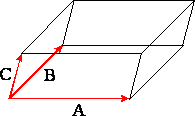
\includegraphics[keepaspectratio = true, scale = 0.3]{rownolegloscian.png}}
						\begin{equation*}
							a(t) = 
							\lim_{\Delta t \to 0} \frac{\Delta v}{\Delta t}
								 = \frac{d v}{d t}
								 = \frac{d}{dt} \left( \frac{d s}{d t} \right)
								 = \frac{d^2 s}{dt^2}
						\end{equation*}	
					
			\item	Styczna do wykresu funkcji $f(x)$ w punkcie $x_0$:
						\begin{equation*}
							y = ax + b, 
								\hspace{10pt} \mathrm{gdzie:} 
								\hspace{20pt} a = f'(x_0),
								\hspace{20pt} b = f(x_0) - f'(x_0) \cdot x_0
						\end{equation*}		
				
		\end{itemize}

		\vspace{7pt}		
		
\subsection{Pochodne funkcji elementarnych}

	\begin{align*}
		(C)' 		&= 0					&	(\sin{x})' 				&= \cos{x}					\\[0.6em]
		(x)' 		&= 1					&	(\cos{x})' 				&= -\sin{x}					\\
		(x^n)' 		&= n x^{n-1}			&	(\tg{x})' 				&= \frac{1}{\cos^2{x}}		\\
		\left( \frac{a}{x} \right)'
					&= \frac{-a}{x^2}		&	(\ctg{x})' 				&= \frac{-1}{\sin^2{x}}		\\
		(\sqrt{x})' &= \frac{1}{2\sqrt{x}} 	& 	(\arcsin{x})' 			&= \frac{1}{\sqrt{1-x^2}}	\\
		\left( a^x \right)' 		
					&= a^x \ln{a} 			&	(\arccos{x})'			&=\frac{-1}{\sqrt{1-x^2}}	\\
		(e^x)' 		&= e^x					&	(\arctg{x})'			&= \frac{1}{x^2+1}			\\
		\left( \log_a{x} \right)' 	
					&= \frac{1}{x\ln{a}}	&	(\arcctg{x})'			&=\frac{-1}{x^2+1}			\\	
		(\ln{x})' 	&= \frac{1}{x}			&	 			&					\\
	\end{align*}



\subsection{Własności}

		\begin{multicols}{2}
		\noindent
			\begin{align*}
				\left[ a \cdot f(x) \right]'  & = a \cdot f'(x)		\\[0.5em]
				\left[ f(x) \pm g(x) \right]' & = f'(x) \pm g'(x) 	\\[0.5em]
				\left[ f(x) \cdot g(x) \right]' 
					& = f'(x) \cdot g(x) + f(x) \cdot g'(x)			\\[0.5em]	
			\end{align*}
			\begin{align*}
				\left[ \frac{f(x)}{g(x)} \right]' & = 
					\frac{f'(x) \cdot g(x) - f(x) \cdot g'(x)}{[g(x)]^2} \\[0.7em]
				\Big[ f \big[ g(x) \big] \Big]'  & = 
						f'\big[ g(x) \big] \cdot g'(x)		
			\end{align*}		
		\end{multicols}



		\newpage
		%%%%%%%%%%%%%%%%%%%%%%%%%%%%%%%
		%%%%%%%%%%%%%%%%%%%%%%%%%%%%%%%	
			\section{Całki}
		%%%%%%%%%%%%%%%%%%%%%%%%%%%%%%%
		%%%%%%%%%%%%%%%%%%%%%%%%%%%%%%%


	%%%%%%%%%%%%%%%%%%%%%%%%%%%%%%%
	\subsection{Wzory podstawowe}
		
		\begin{multicols}{2}
		\noindent
			\begin{alignat*}{2}
			&	\int{0\cdot dx}						&&=C							\\
			&	\int{dx}							&&=x+C						\\
			&	\int{x^{n}\,dx}						&&=\frac{x^{n+1}}{n+1}+C		
													 \hspace{20pt} (n \neq -1)	\\
			&	\int{\frac{1}{x}\,dx}				&&=\ln\left| x \right|+C		\\
			&	\int{\frac{1}{1+x^2}\,dx}			&&=\arctg{x}+C				\\
			&	\int{\frac{1}{\sqrt{1-x^2}}\,dx}	&&=\arcsin x+C	
			\end{alignat*}
			\begin{alignat*}{2}		
			&	\int{a^x\,dx}						&&=\frac{a^x}{\ln a}+C		\\
			&	\int{e^x \, dx}						&&=e^x + C					\\
			&	\int{\sin x\,dx}					&&=-\cos x+C					\\
			&	\int{\cos x\,dx}					&&=\sin x+C					\\
			&	\int{\frac{1}{\sin^2x}\,dx}			&&=-\ctg{x}+C				\\
			&	\int{\frac{1}{\cos^2x}\,dx}			&&=\tg{x}+C			
			\end{alignat*}	
		\end{multicols}
		\vspace{10pt}		
		
		
		
	%%%%%%%%%%%%%%%%%%%%%%%%%%%%%%%
	\subsection{Wzory uogólnione}

		\begin{multicols}{2}
		\noindent
			\begin{alignat*}{2}
				& \int{\frac{dx}{a^2+x^2}}					&&	=\frac{1}{a}\,\arctg{\frac{x}{a}}+C \hspace{20pt} (a \neq 0)				\\[1em]
				& \int{\frac{dx}{\sqrt{a^2-x^2}}}			&& 	=\arcsin{\frac{x}{a}}+C 													\\[1em]
				& \int{\frac{dx}{\sqrt{x^2 \pm a^2}}}		&& 	=\ln{\left|x+\sqrt{x^2 \pm a^2}\right|}+C 									\\[1em]
				& \int{\frac{x\,dx}{\sqrt{a^2 \pm x^2}}}	&& 	= \pm \sqrt{a^2 \pm x^2}+C 													\\[1em]
				& \int{\frac{dx}{a^2-x^2}}					&&	=\frac{1}{2a}\ln{\left|\frac{a+x}{a-x}\right|}+C \hspace{20pt} (a \neq 0) 	\\[1em]
				& \int{\frac{x\,dx}{a^2 \pm x^2}}			&&	=\pm \frac{1}{2}\ln{\left|a^2\pm x^2\right|}+C  							
			\end{alignat*}
			\begin{alignat*}{2}				
				& \int{\frac{f'(x)}{f(x)}\,dx}				&&  =\ln{\left|f(x)\right|}+C 													\\[1em]
				& \int{\frac{1}{\sqrt{ax+b}}\,dx} 			&&  =\frac{2\sqrt{ax+b}}{a} + C 												\\[1em]
				& \int{\frac{f'(x)}{\sqrt{f(x)}}\,dx}		&& 	=2\sqrt{f(x)}+C 															\\[1em]
				& \int{e^{ax}\,dx} 							&&  =\tfrac{1}{a} e^{ax} + C 													\\[1em]
				& \int{\cos{ax}\,dx} 						&& 	=\tfrac{1}{a} \sin{ax} + C 													\\[1em]
				& \int{\sin{ax}\,dx} 						&& 	=-\tfrac{1}{a} \cos{ax} + C 												
			\end{alignat*}	
		\end{multicols}

		\begin{alignat*}{2}	
			& \int{\sqrt{a^2-x^2}}\,dx		&& =\frac{x}{2}\sqrt{a^2-x^2}+\frac{a^2}{2}\arcsin{\frac{x}{a}}+C \hspace{20pt} (a>0)		\\[1em]
			& \int{\sqrt{x^2 \pm a^2}}\,dx	&& =\frac{x}{2} \sqrt{x^2 \pm a^2}+\frac{a^2}{2}\ln{\left|x+\sqrt{x^2 \pm a^2}\right|}+C 	\\[2em]
			& \text{wzór na całkowanie przez części:} \span\span \\[1em]
			& \int{u(x)v'(x)\,dx}			&& =
 			\begin{Vmatrix}
  				u(x)  & v'(x) \\
  				u'(x) & v(x)
 			\end{Vmatrix}					
		=u(x)v(x) - \int{v(x)u'(x)\,dx}
		\end{alignat*}

	\newpage		
	%%%%%%%%%%%%%%%%%%%%%%%%%%%%%%%
	\subsection{Całki funkcji wymiernych}
		
		Wszystkie całki postaci $ \displaystyle \int{\frac{P_n(x)}{Q_m(x)}\,dx} $, gdzie $ P_n(x) $ to wielomian n-tego stopnia, a $ Q_m(x) $ to wielomian m-tego stopnia możemy podzielić na następujące przypadki:
		
		\begin{enumerate}
		
			\item \fbox{$ 	\mathbf{n \ge m} $} \\ \\
				Poprzez dzielenie wielomianu doprowadzamy wyrażenie podcałkowe do postaci: 
				\begin{equation*} 
					\frac{P_n(x)}{Q_m(x)}=
					R_{n-m}(x)+\frac{S_k(x)}{Q_m(x)}, \text{ gdzie } k < m
				\end{equation*} 
				Wyrażenie $ R_{n-m}(x) $ rozwiązujemy standardowym wzorem na całkę z wielomianu, natomiast $ \displaystyle \frac{S_k(x)}{Q_m(x)} $ za pomocą metody z punktu 2. \\
				
			\item \fbox{$ \mathbf{n < m} $} \\ \\
				Doprowadzamy mianownik do postaci iloczynowej (czynników stopnia co najwyżej drugiego) i przedstawiamy go w postaci ułamków prostych:
				\begin{equation*} 
					\frac{A}{(x+a)^k}, \,\, 
					\frac{Ax+B}{(x^2+p \, x+q)^l},
					\hspace{20pt} l,n \in N 
				\end{equation*} 
				
				Na przykład:
				\begin{equation*}
					\int{\frac{1}{x^2(x^2-1)(x^2-x+1)}\,dx}
					=\int{\left(\frac{A}{x} + \frac{B}{x^2}
					+ \frac{C}{x-1} + \frac{D}{x+1} + 
					\frac{Ex+F}{x^2-x+1}\right)\,dx}
				\end{equation*}
				Poszczególne elementy występujące w powyższej całce rozwiązujemy 
				jedną z poniższych metod (gdzie $m$ to stopień wielomianu z
				mianownika, a $n$ to stopień wielomianu z licznika):	
		
		\begin{enumerate}
		
			\item \fbox{$ \mathbf{(m=1)} $} \\ \\ 
				Stosujemy wzór:
			\begin{equation*}
				\int{\frac{1}{x \pm p}\,dx}=\ln\left| x \pm p \right|+C
			\end{equation*}
		
				\item \fbox{$ \mathbf{(m \ge 2) \,\, \wedge \,\, (n=0)} $} \\ \\
				Podstawiamy pod $t$ wyrażenie stojące pod potęgą i korzystamy
				ze wzoru:
				\begin{equation*}
					\int{t^{n}\,dx}=\frac{t^{n+1}}{n+1}+C
				\end{equation*}			
			
			\item \fbox{$ \mathbf{(m=2) \,\, \wedge \,\, (\Delta < 0) \,\, \wedge \,\, (n=0)} $} \\ \\
				Doprowadzamy mianownik do postaci $(x-p)^2 + q$ i po podstawieniu
				$t=x-p$ oraz $q=a^2$ korzystamy ze wzoru:
				\begin{equation*}
					\int{\frac{dt}{a^2+t^2}}=
					\frac{1}{a}\,\arctg{\frac{t}{a}}+C
				\end{equation*}
			
			\item \fbox{$ \mathbf{(m=2) \,\, \wedge \,\, (n=1)} $} \\ \\
				Doprowadzamy licznik do postaci pochodnej mianownika i stosujemy 
				wzory:
				\begin{equation*}
					\int{\frac{f'(x)}{f(x)}\,dx}=
					\ln{\left|f(x)\right|}+C
						\hspace{50pt}
					\int{\frac{dt}{a^2+t^2}}=\frac{1}{a}\,\arctg{\frac{t}{a}}+C
				\end{equation*} \\
				
			\end{enumerate}
		
		\end{enumerate}
		
	\newpage		
	%%%%%%%%%%%%%%%%%%%%%%%%%%%%%%%
	\subsection{Całki funkcji niewymiernych}
		
		Do całek postaci:
%
			\begin{equation*}
				\int{R \left( x,\sqrt[n]{\frac{ax+b}{cx+d}} \right) \, dx}, 
					\hspace{20pt} ad-bc\neq 0
				\end{equation*}
%
		Stosujemy podstawienie typu:
%			
			\begin{equation*}
				t=\sqrt[n]{\frac{ax+b}{cx+d}}, \hspace{10pt} 
				t^n=\frac{ax+b}{cx+d}, \hspace{10pt} x=\varphi(t), \hspace{10pt}
				dx=\varphi'(t)\,dt
			\end{equation*}

		\vspace{40pt}

	%%%%%%%%%%%%%%%%%%%%%%%%%%%%%%%
	\subsection{Całki funkcji trygonometrycznych}


			\begin{enumerate}

			\item Całki typu $ \displaystyle \int{R( \sin{ax} , \cos{bx} )\,dx} $, rozwiązujemy, stosując jeden z następujących wzorów:
				\begin{equation*}
					\begin{split}
		 				\sin\alpha\sin\beta = &
		 					\frac{\cos(\alpha-\beta)-\cos(\beta-\alpha)}{2} \\
						\sin\alpha\cos\beta = &
							\frac{\sin(\alpha-\beta)+\sin(\alpha+\beta)}{2} \\
						\cos\alpha\cos\beta = &
							\frac{\cos(\alpha-\beta)+\cos(\alpha+\beta)}{2} 
					\end{split}
				\end{equation*}


			\item Całki typu $ \displaystyle \int{R( \sin^m x , \cos^n x )\,dx} $ rozwiązujemy stosując jedną z poniższych metod:
			\begin{enumerate}				
			
			\item Podstawienie, gdy funkcja jest nieparzysta względem $ \sin x $: $ t=\cos x $
			\item Podstawienie, gdy funkcja jest nieparzysta względem $ \cos x $: $ t=\sin x $
				\begin{itemize} 
					\item Przykład:
						\begin{equation*}
							\int{\sin^nx \cos^{2k+1}}x\,dx = 
							\int{\sin^nx \cos^{2k}x \cos x\,dx}= 
							\int{\sin^nx(1-sin^2x)^k\,d(\sin x)}
						\end{equation*}
				\end{itemize}				
				
			\item Podstawienie, gdy funkcja jest parzysta wzgledem $ \sin x $, $ \cos x $:
						
		\begin{itemize}
			\item Stosujemy podstawienie:
						\begin{equation*}
							t=\tg{x}, \hspace{10pt}  
							\sin x = \frac{t}{\sqrt{1+t^2}}, \hspace{10pt} 
							\cos x=\frac{1}{\sqrt{1+t^2}}, \hspace{10pt}  
							dx=\frac{dt}{1+t^2}
						\end{equation*}
						
				
						
			\item lub przekształcamy funkcję podcałkową jednym z poniższych wzorów:
						\begin{equation*}
							\sin^2x=\frac{1}{2}(1-\cos2x), \hspace{10pt} 
							\cos^2x=\frac{1}{2}(1+\cos2x), \hspace{10pt}
							\sin x \cos x=\frac{1}{2}\sin2x
						\end{equation*}
						
							
						
		\end{itemize}
			\item Podstawienie, gdy funkcja nie spełnia warunków (a)-(c) (tzw. podstawienie uniwersalne):
						\begin{equation*}
							t=\tg{\frac{x}{2}}, \hspace{10pt} 
							\sin x=\frac{2t}{1+t^2},	 \hspace{10pt} 
							\cos x=\frac{1-t^2}{1+t^2},  \hspace{10pt} 
							dx=\frac{2\,dt}{1+t^2}
						\end{equation*}

		\end{enumerate}
			\end{enumerate}


	\newpage	
	%%%%%%%%%%%%%%%%%%%%%%%%%%%%%%%
	\subsection{Zastosowania w geometrii}

			\begin{enumerate}

				\item Objętość bryły obrotowej powstałej w wyniku obrotu 
					  funkcji dookoła osi OX:
					\begin{itemize}
						\item Funkcja dana jawnie 
							  $ y=y(x), \hspace{10pt} a \le x \le b $			
									\begin{equation*}
										V=\pi \int\limits_a^b{y^2(x)\,dx}
									\end{equation*}		
												
						\item Funkcja dana parametrycznie
							  $ x=x(t), y=y(t),\hspace{10pt} 
							  	\alpha \le t \le \beta $					
									\begin{equation*}
										V=\pi \int\limits_\alpha^\beta{y^2(t)
											| x'(t) | \,dt}
									\end{equation*}						
					\end{itemize}	
					
					
					
				\item Pole powierzchni bryły obrotowej powstałej w wyniku obrotu 
					  funkcji dookoła osi OX:
					\begin{itemize}
						\item Funkcja dana jawnie 
							  $ y=y(x) \ge 0, \hspace{10pt} a \le x \le b $			
									\begin{equation*}
										S = 2\pi \int\limits_a^b
											{y(x) \sqrt{1+\left[y'(x)\right]^2}\,dx}
									\end{equation*}		
												
						\item Funkcja dana parametrycznie
							  $ x=x(t), y=y(t), \hspace{10pt} 
							  	\alpha \le t \le \beta $					
									\begin{equation*}
										S = 2\pi \int\limits_\alpha^\beta
													{y(t) \sqrt{\left[x'(t)\right]^2 		
													+\left[y'(t)\right]^2} \,dt}
									\end{equation*}						
					\end{itemize}				
					
					
					
					
					
				\item Długość łuku funkcji:
					\begin{itemize}
						\item Funkcja dana jawnie 
							  $ y=y(x), \hspace{10pt} a \le x \le b $			
									\begin{equation*}
										L=\int\limits_a^b
											{\sqrt{1+\left[f'(x)\right]^2}
										  \,dx}
									\end{equation*}		
												
						\item Funkcja dana parametrycznie
							  $ x=x(t), y=y(t), \hspace{10pt}
							  	\alpha \le t \le \beta $					
									\begin{equation*}
										L=\int\limits_
											\alpha^\beta
												{\sqrt{\left[x'(t)\right]^2 	
												 + \left[y'(t)\right]^2}
										   \,dt}
									\end{equation*}						
					\end{itemize}				
						
							
				\end{enumerate}
				
		\newpage
		%%%%%%%%%%%%%%%%%%%%%%%%%%%%%%%
		%%%%%%%%%%%%%%%%%%%%%%%%%%%%%%%	
			\section{Geometria Analityczna w 3D}
		%%%%%%%%%%%%%%%%%%%%%%%%%%%%%%%
		%%%%%%%%%%%%%%%%%%%%%%%%%%%%%%%
				
				
\subsection{Wektory}

\begin{itemize}

\item Iloczyn skalarny: \hspace{10pt}	
				$ \vec{a} \cdot \vec{b} 
					= a_x b_x + a_y b_y + a_z b_z
					= |\vec{a}| |\vec{b}| \cos{\varphi} $

\item Iloczyn wektorowy: \hspace{10pt}
				$ \vec{a} \times \vec{b} = 
					\left| 
					\begin{array}{ccc}
						\hat{i} & \hat{j} & \hat{k} \\
						a_x & a_y & a_z \\
						b_x & b_y & b_z 
					\end{array} 
					\right| 
					, \hspace{10pt} 	
					| \vec{a} \times \vec{b}	 | = 
					|\vec{a}| |\vec{b}| \sin{\varphi}	
				$
		\\W wyniku obliczenia iloczynu wektorowego otrzymujemy trzeci
		wektor $\vec{c}$, który jest prostopadły do obydwu wektorów
		$\vec{a}$ oraz $\vec{b}$.

\item Iloczyn mieszany: \hspace{10pt}
				$ \left( \vec{a} \times \vec{b} \right) \cdot \vec{c} = 
					\left| 
					\begin{array}{ccc}
						a_x & a_y & a_z \\
						b_x & b_y & b_z \\
						c_x & c_y & c_z 
					\end{array} 
					\right| 
				$					
					
					
\item Prostopadłość (ortogonalność) wektorów: \hspace{10pt}
				$ \vec{a} \perp \vec{b} 
					\Leftrightarrow 
				  \cos{\varphi} = 0
					\Leftrightarrow
				  \vec{a} \cdot \vec{b} = 0 $
				  
\item Równoległość (kolinearność) wektorów: \hspace{10pt}
				$ \vec{a} \parallel \vec{b} 
					\Leftrightarrow 
				  \sin{\varphi} = 0
					\Leftrightarrow
				  \dfrac{a_1}{b_1} = 
				  \dfrac{a_2}{b_2} = 
				  \dfrac{a_3}{b_3} $		
				
\item Pole równoległoboku zbudowanego na dwóch wektorach: \hspace{10pt}
				$ S = | \vec{a} \times \vec{b} | $
				
\item Pole trójkąta zbudowanego na dwóch wektorach: \hspace{43pt}
				$ S = \tfrac{1}{2} | \vec{a} \times \vec{b} | $
						
\item Objętość równoległościanu zbudowanego na trzech wektorach: \hspace{10pt}
				$ V = | ( \vec{A} \times \vec{B} ) \cdot \vec{C} |			
				\qquad
				\raisebox{-7mm}{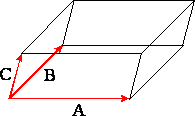
\includegraphics[keepaspectratio = true, scale = 0.3]{rownolegloscian.png}} $
				
\item Objętość czworościanu zbudowanego na trzech wektorach: \hspace{20pt}
				$ \displaystyle
					V = \frac{1}{6}| ( \vec{A} \times \vec{B} ) 
							\cdot \vec{C} |$
				
\item Rzut wektora $\vec{a}$ na wektor $\vec{b}$: \hspace{10pt}
				$ \displaystyle \vec{a}_b = 
					\frac{\vec{a} \cdot \vec{b}}{|\vec{b}|^2} \cdot \vec{b} $			
					
\end{itemize}		


\vspace{30pt}

\subsection{Teoria pola}

		\begin{itemize}
			\item	Gradient pola skalarnego $f$:  \hspace{10pt} 
					$\displaystyle	
						\nabla f(x,y,z) = 
						\left[ 	\frac{\partial f}{\partial x},
								\frac{\partial f}{\partial y},
								\frac{\partial f}{\partial z}   \right] $

			\item	Dywergencja pola wektorowego 
					$\vec{F}=(F_x,F_y,F_z)$:  \hspace{10pt} 
					$\displaystyle	
						\nabla \cdot \vec{F}(x,y,z) = 
							\frac{\partial F_x}{\partial x}
						  + \frac{\partial F_y}{\partial y}
						  + \frac{\partial F_z}{\partial z}  $

			\item	Rotacja pola wektorowego
					$\vec{F}=(F_x,F_y,F_z)$:  \hspace{10pt}
				$ \nabla \times \vec{F}= 
					\left| 
					\begin{array}{ccc}
						\hat{i} & \hat{j} & \hat{k} \\
							\frac{\partial}{\partial x} & \frac{\partial}{\partial y} &	\frac{\partial}{\partial z} \\	
						F_x & F_y & F_z 
					\end{array} 
					\right|	
				$	
				
			\item	Pochodna kierunkowa:  \hspace{10pt} 
					$\displaystyle	
						\nabla_{\vec{u}} f(x_0,y_0,z_0) =
							\frac{\partial f}{\partial \vec{u}} (x_0,y_0,z_0) =
							\nabla f(x_0,y_0,z_0) \cdot \vec{u}	 $
		
				
		
		\end{itemize}

			


%\newpage
\vspace{30pt}


\subsection{Proste}

\begin{itemize}

\item Równanie kierunkowe: \hspace{10pt}
				$ \dfrac{x-x_o}{a} = 
				  \dfrac{y-y_o}{b} = 
				  \dfrac{z-z_o}{c}, \hspace{10pt} 
				  	\text{ gdy } abc \neq 0 $
				 
				 lub	
				$ \left\{
  					\begin{array}{l}
    						x = x_o	\\
    						\frac{y-y_o}{b} = \frac{z-z_o}{c} \\
  					\end{array} \right. 
  					\text{ gdy } a=0 \wedge bc \neq 0 $
  				 \hspace{10pt} oraz analogicznie dla pozostałych.

\item Równanie parametryczne: \hspace{10pt}
				$ \left\{
  					\begin{array}{l}
    						x = x_o + at \\
    						y = y_o + bt \\
    						z = z_o + ct \\
  					\end{array} \right.
  					\qquad
				\raisebox{-11mm}{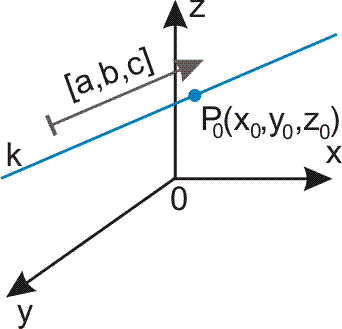
\includegraphics[keepaspectratio = true, scale = 0.2]{prosta.png}} $
  					
  					Prosta wychodząca z punktu $P_o=(x_o,y_o,z_o)$ przeciągnięta przez wektor $\vec{v} = [a,b,c]$
  					
\item Równanie krawędziowe 
		(przecięcie dwóch płaszczyzn nierównoległych)
				
				\hspace{100pt}
				$ l: \left\{
  					\begin{array}{l}
    						A_1 x + B_1 y + C_1 z + D_1 = 0 \\
						A_2 x + B_2 y + C_2 z + D_2 = 0 \\
  					\end{array} \right.
  					\qquad
				\raisebox{-11mm}{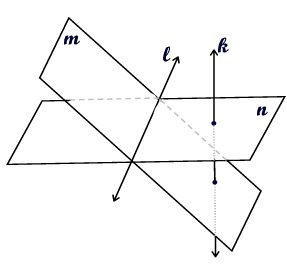
\includegraphics[keepaspectratio = true, scale = 0.4]{krawedziowa.jpg}} $
				  
\item Równanie prostej przechodzącej przez punkty 
		$A$ i $B$:	\hspace{10pt}
				$ \dfrac{x-x_A}{x_A-x_B} = 
				  \dfrac{y-y_A}{y_A-y_B} = 
				  \dfrac{z-z_A}{z_A-z_B} $

\item Wzajemne położenie prostych

		\begin{itemize}
		
			\item 	Prostopadłość: \hspace{10pt}
						$ a_1 a_2 + b_1 b_2 + c_1 c_2 = 0 $
				
			\item 	Równoległość: \hspace{10pt}
						$ 	\dfrac{a_1}{a_2} = 
				  			\dfrac{b_1}{b_2} =
				  			\dfrac{c_1}{c_2} $	
				 
			\item	Przecinanie się: \hspace{10pt}
					$ \vv{P_{01}P_{02}}, \vv{v}_1, \vv{v}_2$ są liniowo
					zależne i nie spełniają warunku równoległości.
					
			\item	Skośność (proste nie leżą w jednej płaszczyźnie): \hspace{10pt}
					$ \vv{P_{01}P_{02}}, \vv{v}_1, \vv{v}_2$ są liniowo
					niezależne.
	
		\end{itemize}


\end{itemize}




%\newpage
\vspace{30pt}

\subsection{Płaszczyzny}

\begin{itemize}

\item Równanie ogólne płaszczyzny: \hspace{10pt}
			$ Ax + By + Cz + D = 0 $
			
			Wektor prostopadły do płaszczyzny 
					$ \vec{R} = [A,B,C] $
					
					Prostopadłość/równoległość płaszczyzn określa
					się przy pomocy prostopadłości/równoległości
					ich wektorów normalnych:
					
				\begin{itemize}
					\item Prostopadłość płaszczyzn:
						$ A_1 A_2 + B_1 B_2 + C_1 C_2 = 0 $ 

					\item Równoległość płaszczyzn:
						$ \dfrac{A_1}{A_2} = 
				  	 	  \dfrac{B_1}{B_2} =
				  	  	  \dfrac{C_1}{C_2} $ 		
				\end{itemize}	

\item Równanie odcinkowe płaszczyzny: \hspace{10pt} 
			$ \dfrac{x}{a} + \dfrac{y}{b} + \dfrac{z}{c} = 1
				\qquad
				\raisebox{-15mm}{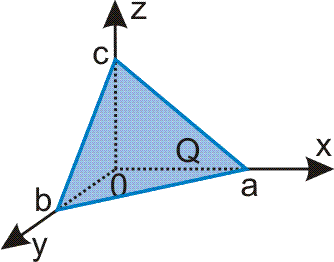
\includegraphics[keepaspectratio = true, scale = 0.3]{plaszczyzna_odcinkowe.png}} $

\vspace{10pt}
\item Równanie płaszczyzny przechodzącej przez 
		3 punkty niewspółliniowe: \hspace{10pt}
			
			\hspace{100pt}
			  $ \left| 
				\begin{array}{ccc}
					x-x_1 & y-y_1 & z-z_1 \\
					x_2-x_1 & y_2-y_1 & z_2-z_1 \\
					x_3-x_1 & y_3-y_1 & z_3-z_1 
				\end{array}
			   \right| = 0 $

\vspace{10pt}
\item Odległość punktu od płaszczyzny: \hspace{10pt}
			$ d = \dfrac{| Ax_o + By_o + Cz_o + D |}
						{\sqrt{A^2 + B^2 + C^2}} $

\vspace{10pt}						
\item Kąt między płaszczyznami 
	 (kąt między wektorami normalnymi do płaszczyzn):
	 		
	 		\hspace{100pt}
	 			$ \cos{\varphi} = 
	 			    \dfrac{\vec{R_1} \cdot \vec{R_2} }
	 			  		  {|\vec{R_1}| |\vec{R_2}|} 	  = 
	 			  	\dfrac{A_1 A_2 + B_1 B_2 + C_1 C_2}
	 			  		  { \sqrt{A_1^2 + B_1^2 + C_1^2}
	 			  		  	\sqrt{A_2^2 + B_2^2 + C_2^2} }$

\vspace{10pt}
\item Płaszczyzna styczna do wykresu funkcji $F(x,y,z)$ 
	  w punkcie $P_o(x_o,y_o,z_o)$: 
	  
	  		\hspace{100pt}
	  			$ F_x(P_o)(x-x_o) + 
	  			  F_y(P_o)(y-y_o) + 
	  			  F_z(P_o)(z-z_o) = 0 $

\end{itemize}


\vspace{35pt}
\subsection{Proste i płaszczyzny}

\begin{itemize}

\item Prostopadłość/równoległość prostej i płaszczyzny:

			\hspace{50pt}
				$ l: \left\{
  						\begin{array}{l}
    							x = x_o + at \\
    							y = y_o + bt \\
    							z = z_o + ct \\
  						\end{array} \right., 
  				\hspace{20pt}
  				  \alpha: Ax + By + Cz + D = 0 $
  			
  			Wektor $\vec{u}(a,b,c)$ jest równoległy do prostej $l$
  			\\Wektor $\vec{R}(A,B,C)$ jest prostopadły do
  			  płaszczyzny $\alpha$ 
  			  
  	\begin{itemize}
  	
  			\item Warunek prostopadłości: 
  			
  			\hspace{50pt}
				$ l \perp \alpha
						\hspace{10pt}
  						\Leftrightarrow
						\hspace{10pt}
  						\vec{u} \parallel \vec{R}
  						\hspace{10pt}
  						\Leftrightarrow
  						\hspace{10pt}
  				  \dfrac{A}{a} = 
				  \dfrac{B}{b} =
				  \dfrac{C}{c} $
				  
			\item Warunek równoległości:
			
			\hspace{50pt}
				$ l \parallel \alpha
						\hspace{10pt}
  						\Leftrightarrow
						\hspace{10pt}
  						\vec{u} \perp \vec{R}
  						\hspace{10pt}
  						\Leftrightarrow
  						\hspace{10pt}
  				  Aa + Bb + Cc = 0 $		
	\end{itemize}
				
\vspace{10pt}	  
\item Punkt przebicia prostej z płaszczyzną
			\\Wyznaczamy parametr $t$ podstawiając $l$ do $\alpha$:
				$ A(x_o + at) + B(y_o + bt) + C(z_o + ct) + D = 0 $
			\\Współrzędne punktu przebicia otrzymamy podstawiając 
			  parametr $t$ do równania prostej $l$.
			  
\vspace{10pt}	  
\item Kąt nachylenia prostej do płaszczyzny: \hspace{10pt}
			$ \sin{\varphi} = 
				\dfrac{|Aa+Bb+Cc|}
					  { \sqrt{A^2 + B^2 + C^2}
	 			  		\sqrt{a^2 + b^2 + c^2} } $



\end{itemize}	


		\newpage
		%%%%%%%%%%%%%%%%%%%%%%%%%%%%%%%
		%%%%%%%%%%%%%%%%%%%%%%%%%%%%%%%	
			\section{Elementy Trygonometrii Sferycznej}
		%%%%%%%%%%%%%%%%%%%%%%%%%%%%%%%
		%%%%%%%%%%%%%%%%%%%%%%%%%%%%%%%

\subsection{Podstawowe informacje}
	
			\begin{itemize}
				\item 	Trygonometria sferyczna zajmuje się związkami w trójkątach 
						na powierzchni kuli, czyli tzw. trójkątach sferycznych. 
						Trójkąt sferyczny jest figurą, której bokami są łuki 
						kół wielkich przechodzące przez każdą z par spośród trzech
						punktów będących jego wierzchołkami. Poniżej znajdują
						się dwa przykładowe trójkąty sferyczne.
											
					\vspace{5pt}	
					\begin{figure}[h!]
						\centering
						\begin{subfigure}{.5\textwidth}
							\centering
  							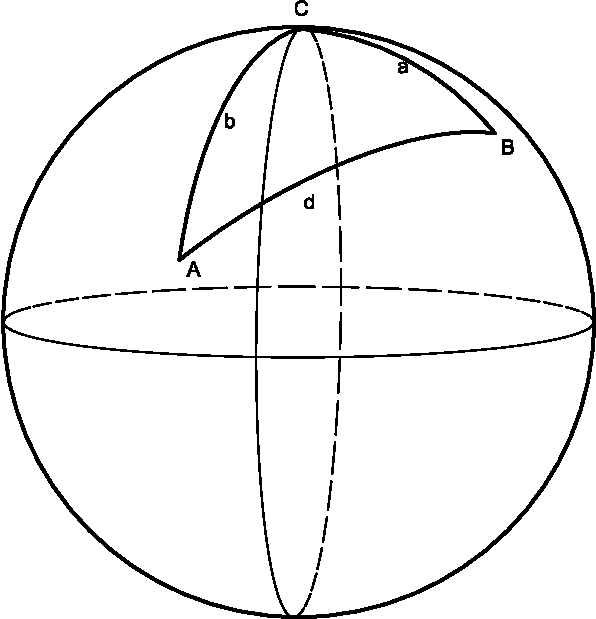
\includegraphics[height=140pt]
  											{trojkat_sferyczny1.pdf}
						\end{subfigure}%
						\begin{subfigure}{.5\textwidth}
							\centering
  							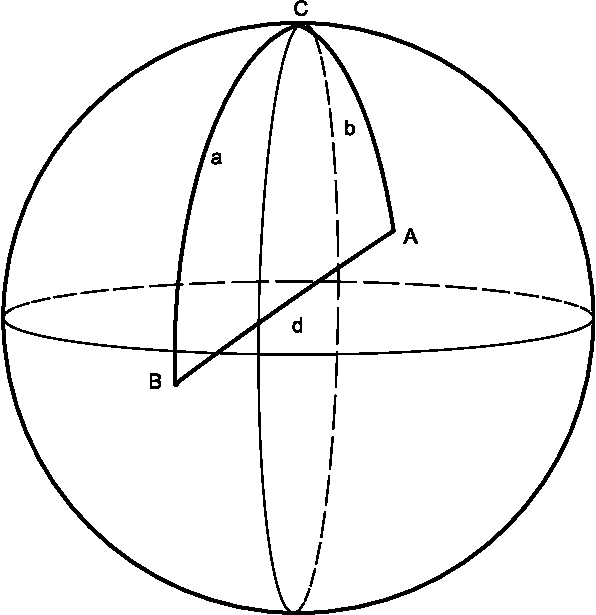
\includegraphics[height=140pt]
  											{trojkat_sferyczny2.pdf}							
						\end{subfigure}
					\end{figure}

					
				\item 	W trójkącie sferycznym miarą zarówno kątów $A,B,C$ jak i 
						boków $a,b,d$ są stopnie. Jego boki są łukami
						wyrażonymi w mierze swoich kątów środkowych.
				
				\vspace{-2pt}		
				\item 	Podstawowe własności trójkątów sferycznych:
				\vspace{-3pt}
				\begin{itemize}	
					\item	Każdy element trójkąta sferycznego jest mniejszy 
							od $180\degree$,
					\item	$	0\degree < a+b+c < 180\degree, 
									\hspace{20pt}
								180\degree < A+B+C < 540\degree		$,
					\item	Naprzeciw dłuższego boku leży większy kąt.
				\end{itemize}
				
				\vspace{-2pt}		
				\item	W celach nawigacyjnych rozważane trójkąty sferyczne będą
						posiadały jeden wierzchołek $(C)$ na biegunie północnym.
						Boki $a,b$ leżą na południkach przechodzących odpowiednio
						przez punkty $B,A$.
				
				\vspace{-2pt}
				\item	Ortodroma jest krótszym łukiem koła wielkiego przechodzącego
						przez dwa punkty na sferze i wyznacza najkrótszą drogę między
						nimi (tzw. odległość ortodromiczną między punktami $A$ i $B$
						oznaczoną jako $d$).
						Jest ona zawsze wygięta w kierunku bliższego bieguna.
				
				\vspace{-2pt}		
				\item	Kąty drogi są mierzone zawsze względem ruchu wskazówek
						zegara, między południkiem przechodzącym przez dany punkt
						a dodatnim kierunkiem ruchu. Szczegółowo jest to
						zobrazowane na rysunkach na stronie \pageref{fig:e-w}.
						Są na nich zaznaczone wszystkie elementy zarówno
						trójkąta sferycznego jak i samej ortodromy,
						które musimy wyznaczyć.	
				
				\vspace{-2pt}	
				\item	Aby poruszać się po ortodromie, kąt drogi musi być cały
						czas zmieniany (poza przypadkiem poruszania się po równiku -
						wtedy kąt drogi wynosi stale $90\degree$ lub $270\degree$, 
						lub po dowolnym południku - wtedy kąt drogi wynosi stale 
						$0\degree$ lub $180\degree$).
				
				\vspace{-2pt}		
				\item	Wierzchołki ortodromy to dwa punkty $W_1$ oraz $W_2$
						leżące na kole wielkim zawierającym daną ortodromę, 
						wysunięte najbardziej na północ oraz 
						najbardziej na południe.
				
				\vspace{-2pt}		
				\item	współrzędne geograficzne składają się z szerokości
						geograficznej (N,S) podawanej w zakresie 
						$[-90\degree;90\degree]$.
						(jako odchylenie na północ lub południe od równika) oraz
						z długości geograficznej (E,W) podawanej w zakresie 
						$[-180\degree;180\degree]$ (jako odchylenie na wschód 
						lub zachód od południka zerowego).
					
						\begin{figure}[h!]
							\centering
							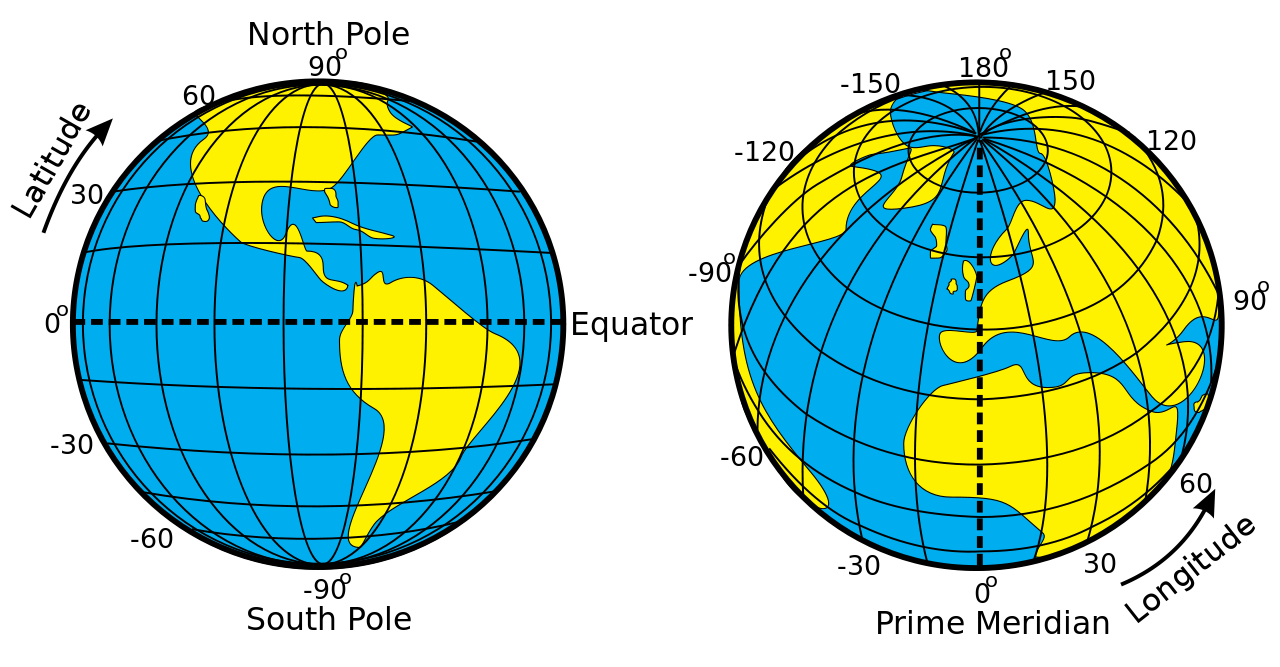
\includegraphics[height=120pt]
											{wspolrzedne.png}
						\end{figure}					
						
			\end{itemize}
				
				
\subsection{Twierdzenie cosinusów (dla boków)}	\label{tw_cos}

			\begin{itemize}
				\item	W dowolnym trójkącie sferycznym $ABCabd$ możemy
						zdefiniować następujące wzory:
					%%
					\begin{align*}
						\cos{a} & = \cos{b} \cos{d} +	\sin{b} \sin{d} \cos{A}	\\
						\cos{b} & = \cos{a} \cos{d} +	\sin{a} \sin{d} \cos{B}	\\
						\cos{d} & = \cos{a} \cos{b} +	\sin{a} \sin{b} \cos{C}  
				\end{align*}							
			\end{itemize}						


\subsection{Reguła Nepera}	\label{regula_nepera}

			\begin{itemize}
				\item 	W celu znalezienia wysokości trójkąta sferycznego oraz
						miary kąta przylegającego do niej 
						można skorzystać z tzw. reguły Nepera. Poniżej znajdują
						się przykładowe rysunki dla przypadków kiedy wysokość
						trójkąta znajduje się wewnątrz trójkąta oraz poza nim.
					\\
						\begin{figure}[h!]
  							\centering
  							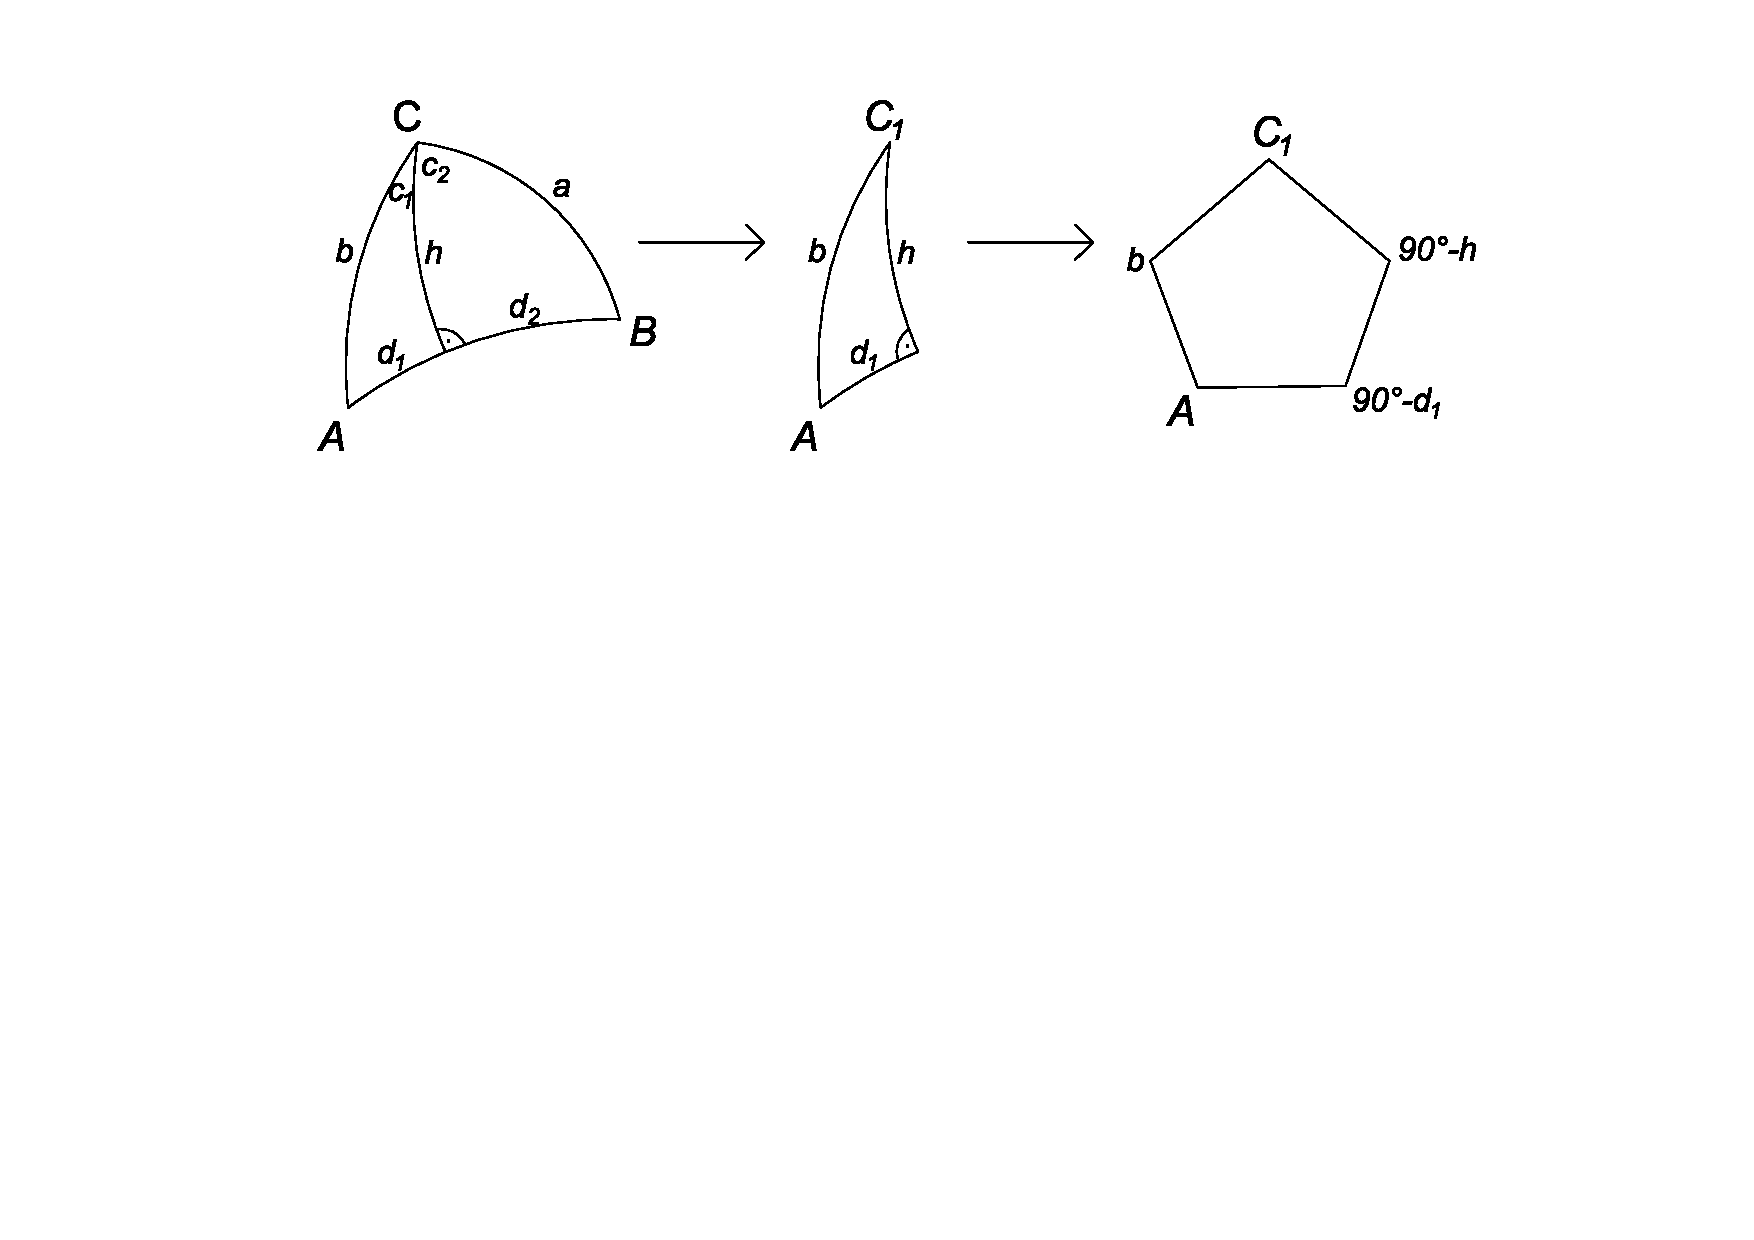
\includegraphics[width=0.65\textwidth]
  											{neper_wew.pdf}
						\end{figure}

						\begin{figure}[h!]
  							\centering
  							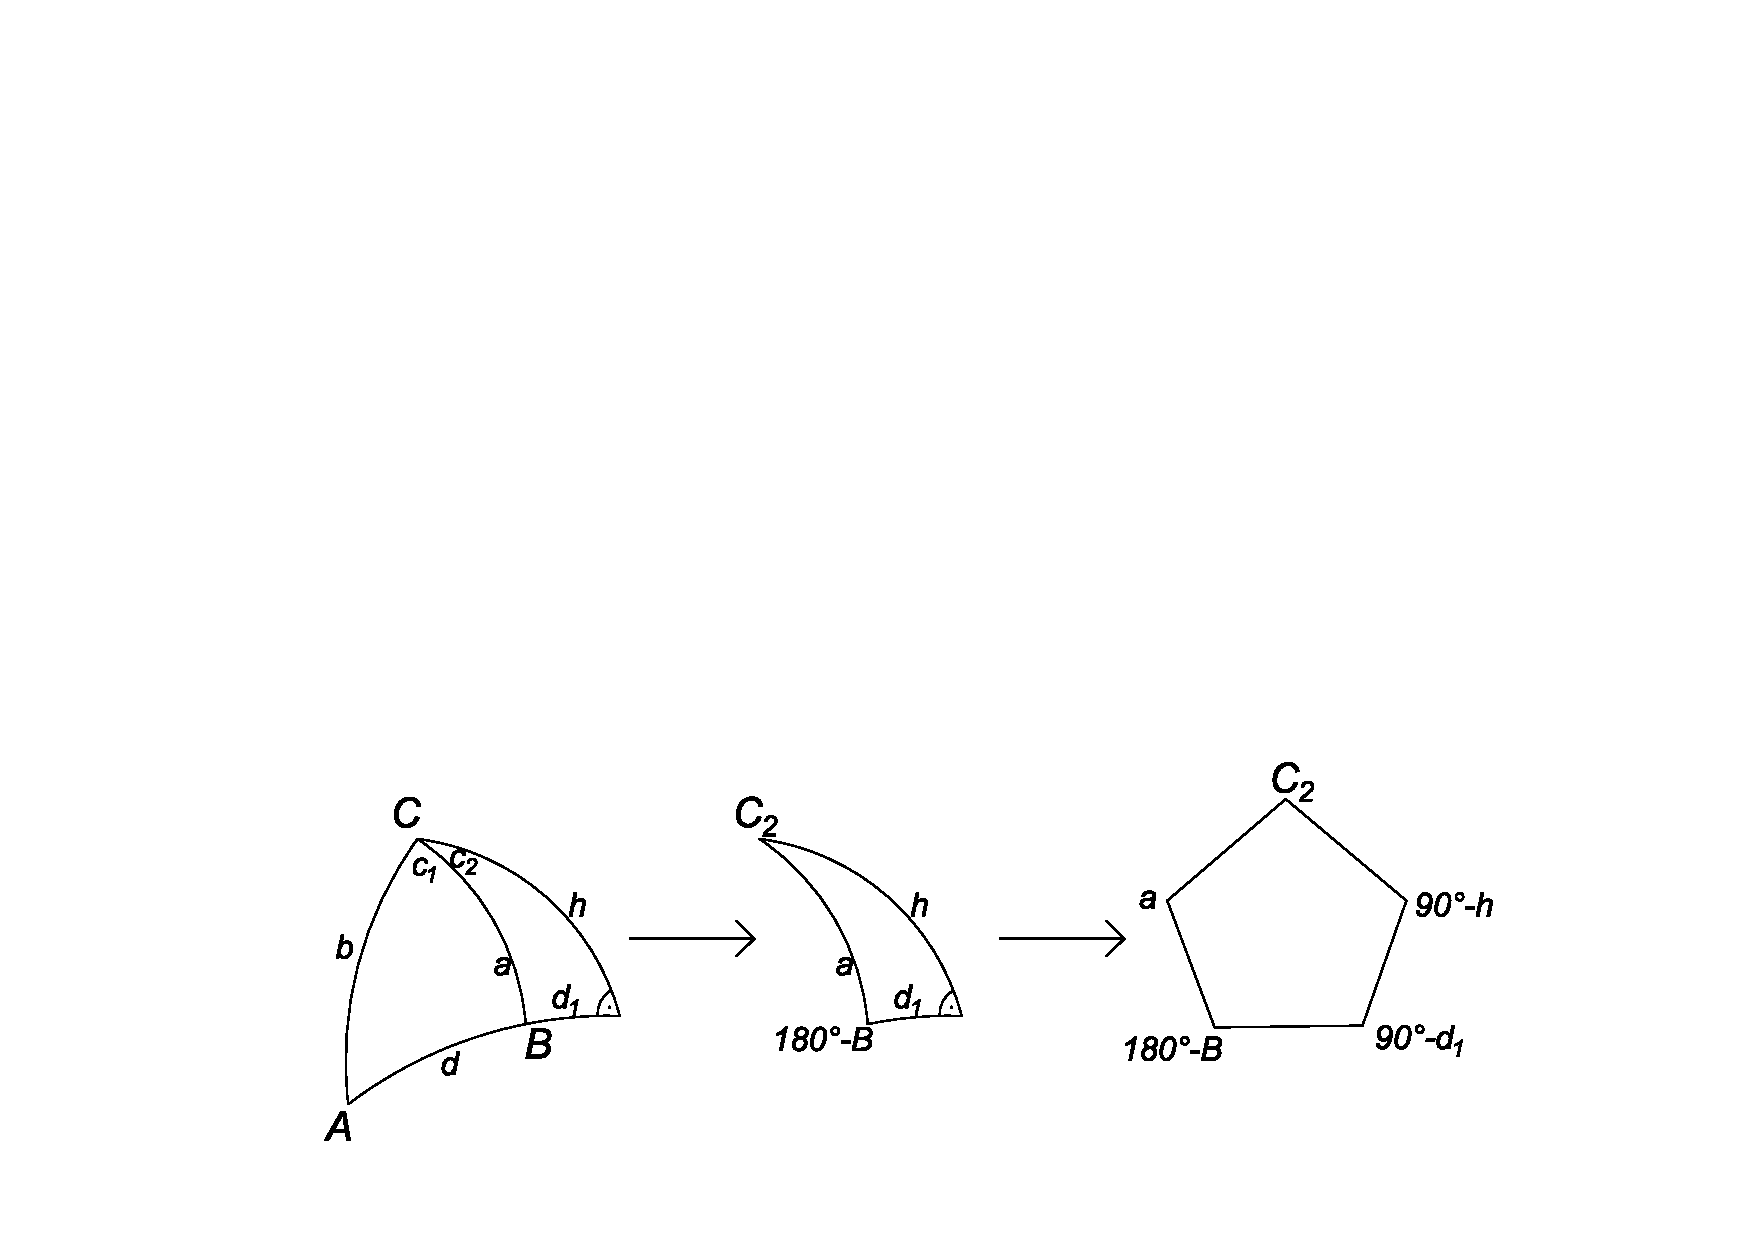
\includegraphics[width=0.65\textwidth]
  											{neper_zew.pdf}
						\end{figure}	
					
				\item 	Jeśli rozmieścimy pięć elementów prostokątnego trójkąta
						sferycznego na pięciokącie (pomijając kąt prosty) w takiej 
						kolejności, w jakiej występują w trójkącie i zastąpimy 
						przy tym przyprostokątne ich dopełnieniami 
						do $90\degree$, to:
						\begin{itemize}
							\item 	cosinus każdego z elementów jest równy 
									iloczynowi cotangensów dwóch przylegających 
									do niego elementów,
							\item	cosinus każdego z elementów jest równy 
									iloczynowi sinusów dwóch nieprzylegających 
									do niego elementów.
									
						\end{itemize}	
												
									W szczególności (na podstawie górnego
									rysunku):
								%%								
								\begin{alignat*}{6}
		\cos{(90\degree - h)}	&= \sin{b} \cdot \sin{A} 
				&&\hspace{20pt}\Rightarrow\hspace{10pt}
					\sin{h} &&= \sin{b} \cdot \sin{A}		\\
		\cos{b	}				&= \ctg{C_1} \cdot \ctg{A}
				&&\hspace{20pt}\Rightarrow\hspace{10pt}
					\cos{b}  &&= \frac{1}{\tg{C_1} \cdot \tg{A}}	
				&&\hspace{20pt}\Rightarrow\hspace{10pt}
					\tg{C_1} &&= \frac{1}{\cos{b} \cdot \tg{A}}							
								\end{alignat*}							
				
				\vspace{-\baselineskip}
				\item	Do rozwiązania powyższych równań zastosowano
						m.in. wzór $\displaystyle
								\ctg{\alpha} = \frac{1}{\tg{\alpha}}$ 
						oraz wzory redukcyjne:
		%%			
		\begin{multicols}{2}
		\noindent
			\begin{align*}
				\sin{(90\degree - \alpha)} 	& = \cos{\alpha}		\\
				\cos{(90\degree - \alpha)} 	& = \sin{\alpha}		\\
				\ctg{(90\degree - \alpha)} 	& = \tg{\alpha}		
			\end{align*}
			\begin{align*}
				\sin{(180\degree - \alpha)} & =  \sin{\alpha}		\\
				\cos{(180\degree - \alpha)} & = -\cos{\alpha}		\\
				\ctg{(180\degree - \alpha)} & = -\ctg{\alpha}			
			\end{align*}		
		\end{multicols}
	
				\end{itemize}
	
\subsection{Algorytm rozwiązania zadania metodą klasyczną}

		\begin{itemize}
				\item	Na wejściu otrzymujemy współrzędne geograficzne dwóch
						punktów (początkowego i końcowego). Przykładowo:
		
							$ A(52\degree 46' \mathrm{ S} ; 
								73\degree 24' \mathrm{W}) ;
								\hspace{10pt}
		  					  B(34\degree 54' \mathrm{S} ; 
		  						95\degree 00' \mathrm{E}) $
										
						Celem zadania jest wyznaczenie odległości ortodromicznej 
						($d$) pomiędzy nimi, początkowego
						kąta drogi ($\alpha$), końcowego kąta drogi ($\beta$) oraz
						współrzędnych wierzchołków ortodromy $W_1$ i $W_2$.		
	
		\end{itemize}

		\newpage
		\textbf{ETAPY ROZWIĄZANIA:}
		
		\begin{enumerate}
				\item	Zamieniamy współrzędne geograficzne obu punktów na 
						wartości liczbowe szerokości ($\varphi$) oraz długości
						geograficznych ($\lambda$) korzystając z przyjętej 
						konwencji znaków: (+) dla NE, (-) dla SW.
						
				\item	Rysujemy rzut równikowy (jest on przedstawiony na
						\pageref{fig:e-w}. stronie) i zaznaczamy 
						długości geograficzne
						obu punktów (w celu sprawdzenia w którą stronę będzie
						krótsza droga: $ W \rightarrow E$ czy $ E \rightarrow W$).
						Kierunek drogi łatwo jest również
						ustalić na podstawie płaskiego
						odwzorowania Ziemi. Droga na wschód zawsze będzie na nim
						odwzorowana jako droga w prawo.
						\\UWAGA: Nawet płynąc
						w prawo ze wschodniej półkuli na zachodnią (przecinając
						południk $180\degree$) jest to traktowane jako droga z
						zachodu na wschód. Analogicznie jest dla 
						przeciwnego kierunku.
					
						\vspace{10pt}
						\begin{figure}[h!]
						\centering
  							\tiny{180\degree W 	\hspace{30pt} 
  							0\degree		\hspace{30pt}
  							180\degree E \\}
  							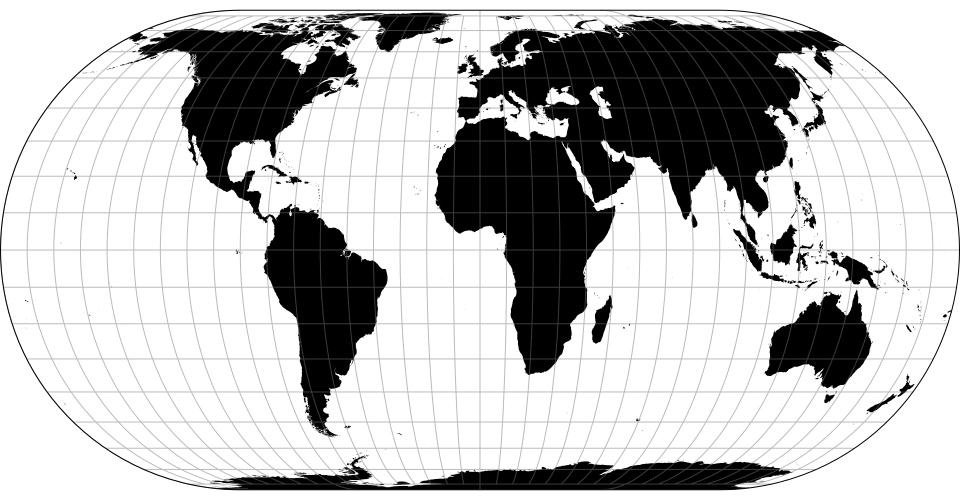
\includegraphics[height=95pt]
  											{mapa_plaska.png}
  							\\
  							\tiny{180\degree W 	\hspace{30pt} 
  							0\degree		\hspace{30pt}
  							180\degree E \\}
						\end{figure}	
						\vspace{10pt}
						
				\item	Wyznaczamy $a,b,C$ (przyjmujemy 
						$\Delta \lambda = \lambda_B - \lambda_A$):
						%%
						\begin{multicols}{2}
						\noindent							
							\begin{align*}
									a & = 90\degree - \varphi_B \\
									b & = 90\degree - \varphi_A
							\end{align*}
							\begin{align*}
								C = & \left\{
  						\begin{array}{ll}
    							|\Delta \lambda|
    								& \mathrm{gdy}  |\Delta \lambda| \le 180\degree  \\
    							360\degree - |\Delta \lambda|
    								& \mathrm{gdy}  |\Delta \lambda| > 180\degree
  						\end{array} \right.
  							\end{align*}	
						\end{multicols}								
								
				\item	Wyznaczamy odległość ortodromiczną z twierdzenia cosinusów
						(\ref{tw_cos}).
						Aby wyznaczyć ją w milach morskich (Mm) mnożymy otrzymany w
						stopniach wynik przez $60$.
						
				\item	Wyznaczamy miary kątów $A,B$ - z twierdzenia cosinusów
						(\ref{tw_cos}),
						po wyznaczeniu z odpowiednich równań cosinusów kątów:
						%%			
						\begin{multicols}{2}
						\noindent
						$$
							\cos{A} = 
								\frac{\cos{a}-\cos{b}\cos{d}}
									 {\sin{b}\sin{d}}
						$$
						$$ 
							\cos{B} = 
								\frac{\cos{b}-\cos{a}\cos{d}}
									 {\sin{a}\sin{d}}						
						$$
						\end{multicols}
			
				\item	Obliczamy początkowy oraz końcowy kąt drogi:


						\begin{multicols}{2}
						\noindent
							\begin{align*}	
								W \rightarrow E & : \left\{
  						\begin{array}{l}
    							\alpha = A				\\
    							\beta  = 180\degree - B \\
  						\end{array} \right.	
 							\end{align*}
 							\begin{align*}
								E \rightarrow W & : \left\{
  						\begin{array}{l}
    							\alpha = 360\degree - A	\\
    							\beta  = 180\degree + B \\
  						\end{array} \right.				
							\end{align*}						
						\end{multicols}
												
				\item	Wprowadzamy do naszego trójkąta $ABCabd$ wysokość $h$
						wychodzącą z wierzchołka $C$ i obliczamy wartości $C_1$
						(lub $C_2$)
						oraz $h$ korzystając z reguły Nepera 
						(\ref{regula_nepera}). Jeżeli kąty $A,B$
						są jednorodne (oba rozwarte lub oba ostre) to wysokość $h$
						będzie leżała wewnątrz trójkąta, a jeżeli są niejednorodne
						to wysokość będzie leżała na zewnątrz, po stronie kąta
						rozwartego.
						Wysokość $h$ przecina koło wielkie naszej 
						ortodromy w punkcie będącym jej	wierzchołkiem $W_1$.
						\\UWAGA: Przy wyznaczaniu dowolnej wielkości z funkcji
						$\sin{h}$ otrzymujemy dwa możliwe rozwiązania: $(h)$ oraz 
						$(180\degree - h)$. Na podstawie własności trójkąta
						sferycznego wybieramy jedyne właściwe rozwiązanie. Często
						wystarczy zauważenie na podstawie rysunku, 
						czy wysokość powinna być większa
						czy mniejsza niż $90\degree$ (czyli na której półkuli
						spodziewamy się wierzchołka $W_1$).			
						
				\item	Obliczamy wierzchołki ortodromy wykorzystując podane
						wzory, a następnie zaznaczamy długości
						$\lambda_{W_1}$ oraz
						$\lambda_{W_2}$ na rzucie równikowym
						(rysunek na stronie obok):
						%%
						\begin{multicols}{2}
						\noindent
						\begin{align*}	
								W_1 & = \left\{
  						\begin{array}{l}
    							\varphi_{W_1} 	= 90\degree - h					\\
    							\lambda_{W_1}	= \lambda_A \pm C_1 
    											  \hspace{5pt} \vee \hspace{5pt}
    											  \lambda_B \pm C_2				\\
  						\end{array} * \right.
						\end{align*}
  						\begin{align*}
								W_2 & = \left\{
  						\begin{array}{l}
    							\varphi_{W_2} 	= -\varphi_{W_1}				\\
    							\lambda_{W_2}	= \lambda_{W_1} \pm 180\degree	\\
  						\end{array} ** \right.				
							\end{align*}
						\end{multicols}
						%
						* Prawidłową zależność wybieramy na podstawie rysunku, 
						biorąc pod uwagę odchylenie wysokości (o kąt $C_1$ lub
						$C_2$) od odpowiedniego południka (biegnącego do punktu
						$A$ lub $B$).
							\\		\\				
						** Tak, aby $\lambda_{W_2} \in [-180\degree,180\degree]$
						- czyli aby miała sens długości geograficznej.
								
		\end{enumerate}

		\newpage
		
\subsection{Rysunki szczegółowe}	

					\vspace{25pt}
							
					\begin{figure}[h!]
						\centering
						\begin{subfigure}{.5\textwidth}
  							\begin{flushleft}
  							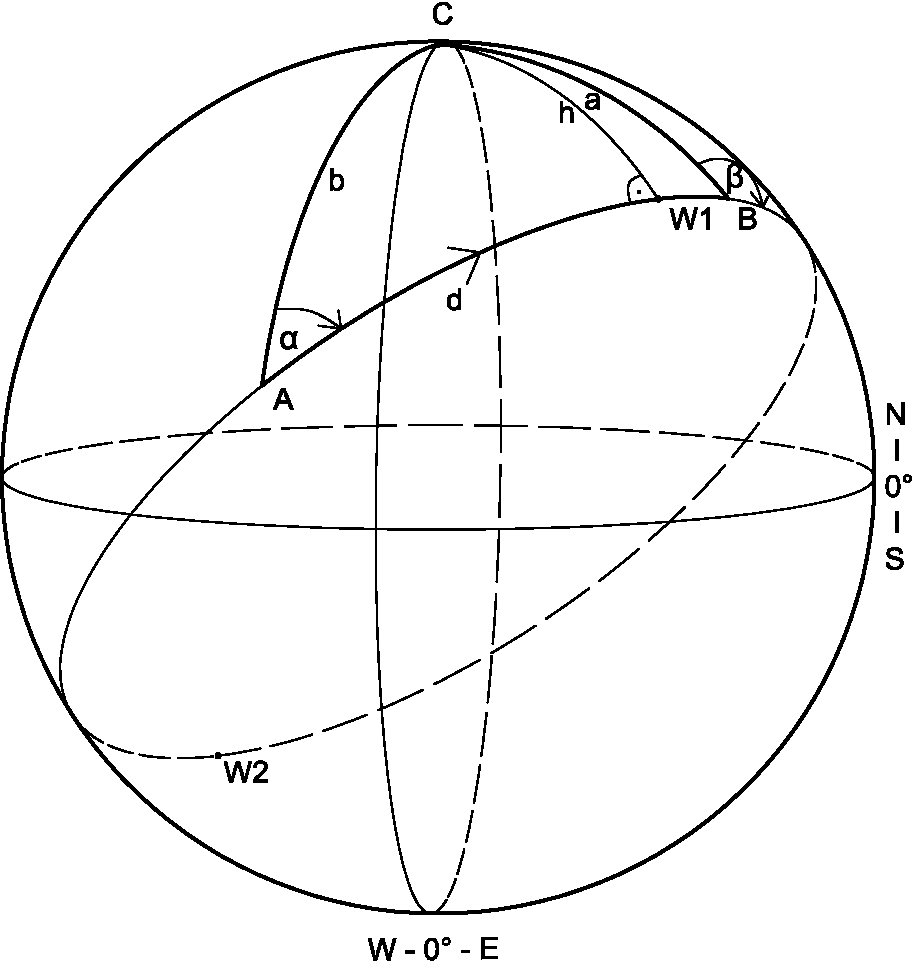
\includegraphics[height=250pt]
  											{katy_WE.pdf}
  							\end{flushleft}
						\end{subfigure}%
						\begin{subfigure}{.5\textwidth}
						  	\begin{flushright}
  							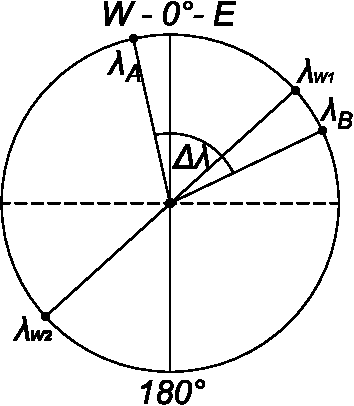
\includegraphics[height=150pt]
  											{rzut_rownik_WE.pdf}							
  							\end{flushright}
						\end{subfigure}
						 \caption{Kompletny rysunek przy
  								  kursie W$\longrightarrow$E wraz z
  								  rzutem równikowym}
  						 \label{fig:w-e}
					\end{figure}	
						
					\vspace{50pt}	
					
					\begin{figure}[h!]
						\centering
						\begin{subfigure}{.5\textwidth}
  							\begin{flushleft}
  							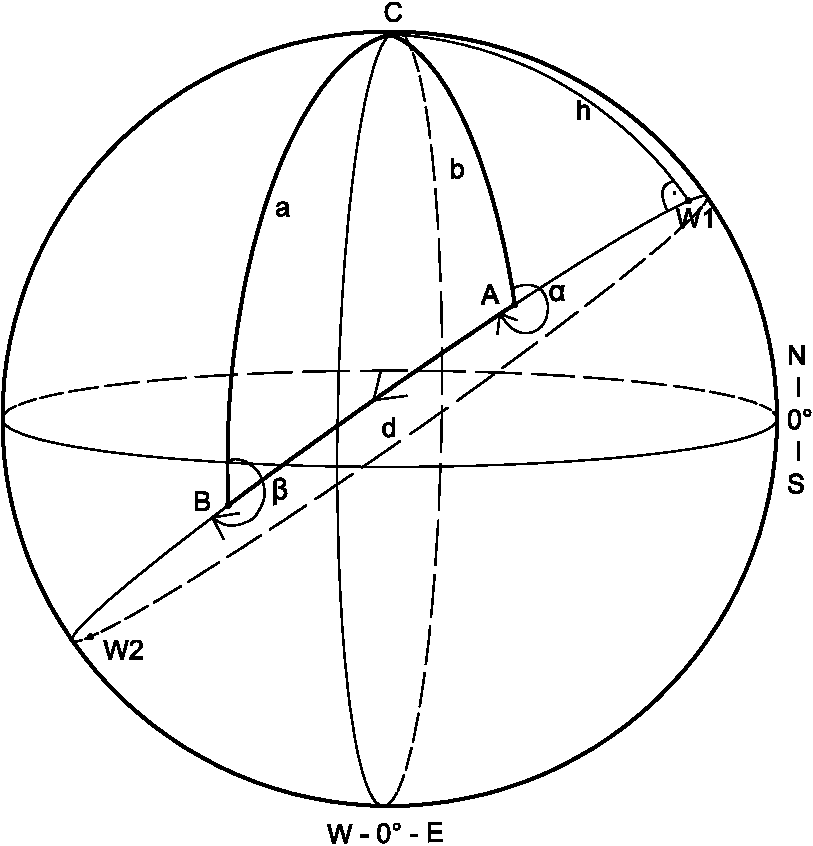
\includegraphics[height=250pt]
  											{katy_EW.pdf}
  							\end{flushleft}
						\end{subfigure}%
						\begin{subfigure}{.5\textwidth}
						  	\begin{flushright}
  							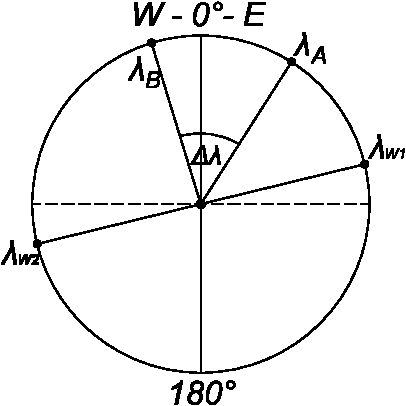
\includegraphics[height=150pt]
  											{rzut_rownik_EW.pdf}							
  							\end{flushright}
						\end{subfigure}
						 \caption{Kompletny rysunek przy
  								  kursie E$\longrightarrow$W wraz z
  								  rzutem równikowym}
  						 \label{fig:e-w}
					\end{figure}	
			
%% Pusta strona na koniec
		\newpage
		\leavevmode
		\thispagestyle{empty}
		\newpage
			
	
\end{document}
